\begin{comment}
\section{Edycja danych}

Po zapisaniu najnowszych danych, następnym krokiem jest wprowadzenie niezbędnych aktualizacji dotyczących usług. W związku z tym utworzono dwa ekrany -- pierwszy służy do wyboru usługi z listy, a drugi przedstawia niezbędne szczegóły oraz umożliwia edycję związanych z nią informacji.

\subsection{Ekran wyboru usługi do edycji}

\begin{figure}[h]
    \centering
    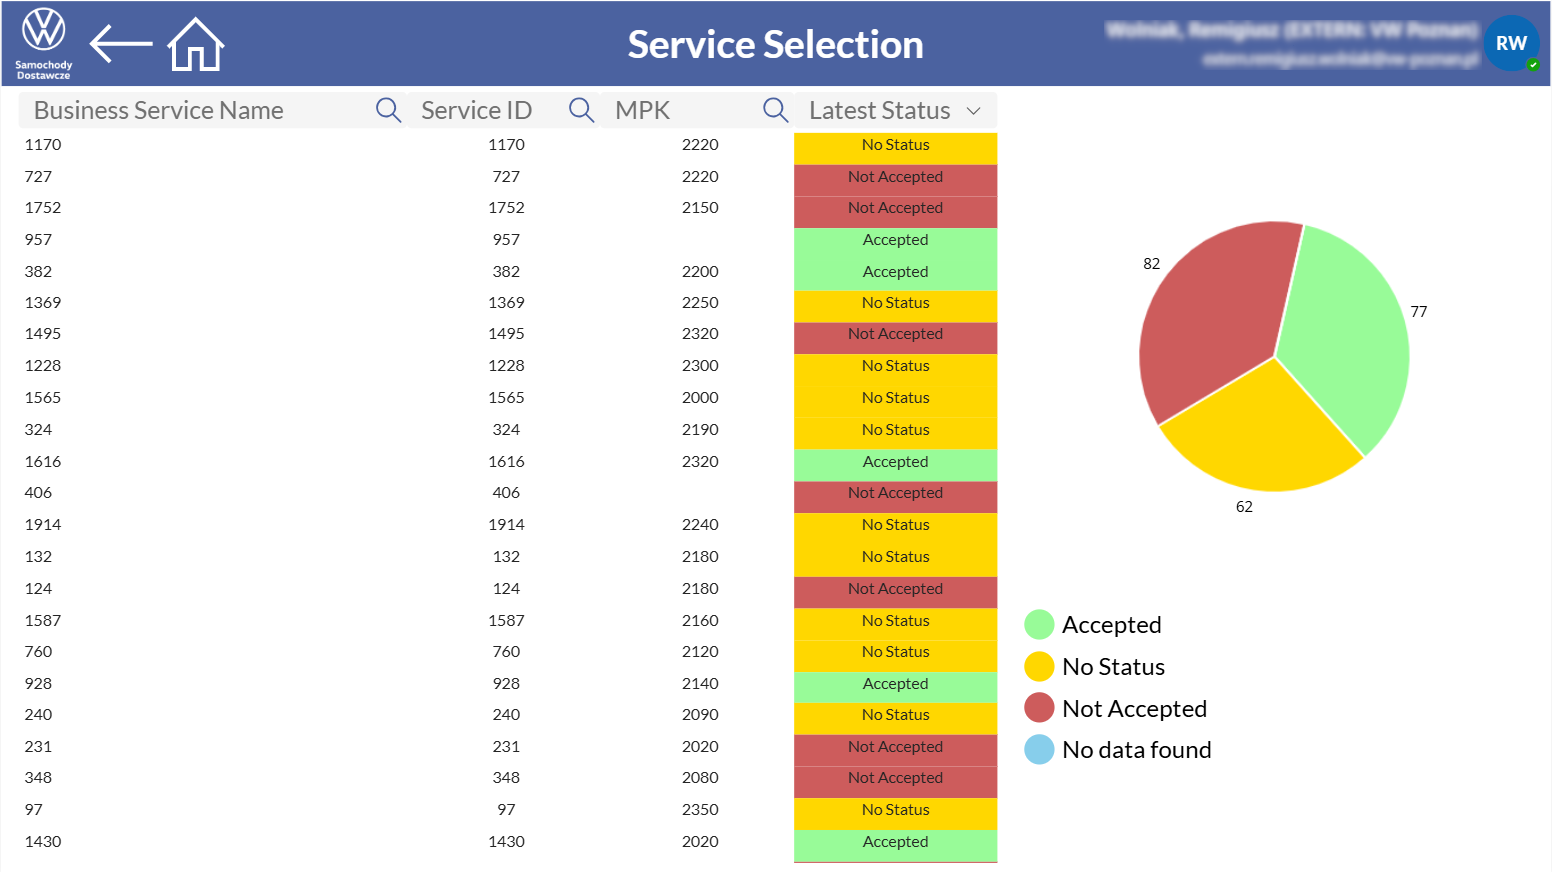
\includegraphics[width=0.9\textwidth]{figures/ServiceSelectionForm.png}
    \caption{Ekran wyboru usługi do edycji}  
    \label{fig:ServiceSelectionForm}
\end{figure}
\end{comment}
\begin{comment}

Ekran wyboru elementu do obróbki składa się z: \begin{enumerate}
%     \item listy, przedstawiającej dane z tymczasowej kolekcji \textit{MergedData}, utworzonej specjalnie na potrzeby obsługi wyboru danych do edycji,
%     \item pól wyszukiwania i filtrów, umożliwiających zawężenie listy na podstawie nazwy usługi, identyfikatora (\textit{Service ID}), miejsca powstawania kosztów (\textit{MPK}) oraz statusu decyzji (\textit{Accepted}, \textit{Not Accepted}, \textit{No Status}),
%     \item wykresu kołowego, prezentującego wizualne podsumowanie liczby elementów w każdej kategorii statusu decyzji,
%     \item interfejsu umożliwiającego dynamiczne dopasowanie wyników listy w czasie rzeczywistym, na podstawie wprowadzonych kryteriów wyszukiwania,
     \item nagłówka, który przedstawia kontekst użytkownika, w tym nazwę i dane aktualnie zalogowanego użytkownika. \end{enumerate}
\end{comment}
\begin{comment}
\subsubsection*{Lista wyboru serwisu}
Lista prezentuje dane pochodzące z dynamicznej kolekcji \textit{MergedData}, która została utworzona w celu zintegrowania informacji z trzech różnych list SharePoint (\textit{Lista\_Uslug}, \textit{Lista\_Kwot}, \textit{Lista\_Indykacji}). Dzięki zastosowaniu wbudowanych funkcji \textit{LookUp} (wyszukiwanie pojedynczego elementu w źródle danych na podstawie warunku) oraz \textit{AddColumns} (dodawanie nowych kolumn do istniejącego źródła danych), dane są filtrowane tak, aby wyświetlać jedynie najnowsze rekordy, np. dla najświeższych decyzji i kwot. Taka struktura zapewnia użytkownikom dostęp do aktualnych informacji bez konieczności ręcznego przeszukiwania źródłowych list. Lista jest dynamiczna, co oznacza, że zmiany w danych źródłowych są automatycznie uwzględniane.

Każdy element na liście posiada dodatkową funkcję interakcji. Po najechaniu kursorem na wybraną usługę (funkcja \textit{hover}), element wizualnie zmienia swój wygląd -- zwęża się, zmienia kolor oraz staje się możliwy do kliknięcia. Kliknięcie przenosi użytkownika do dedykowanego ekranu edycji, który umożliwia szczegółowe zarządzanie wybraną usługą.

\subsubsection*{Pola wyszukiwania i filtry}
Użytkownik ma możliwość zawężenia widocznych danych poprzez zastosowanie różnych kryteriów wyszukiwania. Pola obejmują:
\begin{itemize}
    \item {Wyszukiwanie po nazwie usługi (\textit{Service Name})} -- Obsługuje częściowe dopasowania dzięki wbudowanej funkcji \textit{StartsWith} (sprawdza, czy ciąg tekstowy zaczyna się od określonej frazy).
    \item {Filtrowanie po identyfikatorze usługi (\textit{Service ID})} -- Umożliwia precyzyjne wyszukiwanie konkretnego elementu.
    \item {Filtrowanie według miejsca powstawania kosztów (\textit{MPK})} -- Pozwala na szybkie odnalezienie danych przypisanych do konkretnego obszaru finansowego.
    \item {Filtrowanie według statusu decyzji (\textit{Accepted}, \textit{Not Accepted}, \textit{No Status})} -- Dzięki zastosowaniu funkcji \textit{Switch} (zwraca wartość w zależności od spełnionego warunku), wartości statusów są mapowane na odpowiednie kody liczbowe.
\end{itemize}
Filtry te mogą być stosowane jednocześnie, co umożliwia precyzyjne dopasowanie wyświetlanych danych.

\subsubsection*{Wykres kołowy}
Wykres kołowy ilustruje podział danych według statusów decyzji. Każdy segment odpowiada liczbie elementów z przypisanym statusem, co pozwala użytkownikowi szybko ocenić proporcje między kategoriami (\textit{Accepted}, \textit{Not Accepted}, \textit{No Status}). Wykres jest dynamiczny -- aktualizuje się w czasie rzeczywistym w oparciu o zastosowane filtry.



\subsection{Ekran edycji elementu}
Ekran edycji elementu, widoczny na rysunku \ref{fig:EditForm}, prezentuje szczegółowe informacje dotyczące wybranej usługi, umożliwiając analizę danych historycznych oraz wprowadzanie nowych decyzji. Ekran składa się z kilku logicznie ułożonych sekcji, które są opisane poniżej.
\begin{figure}[h]
    \centering
    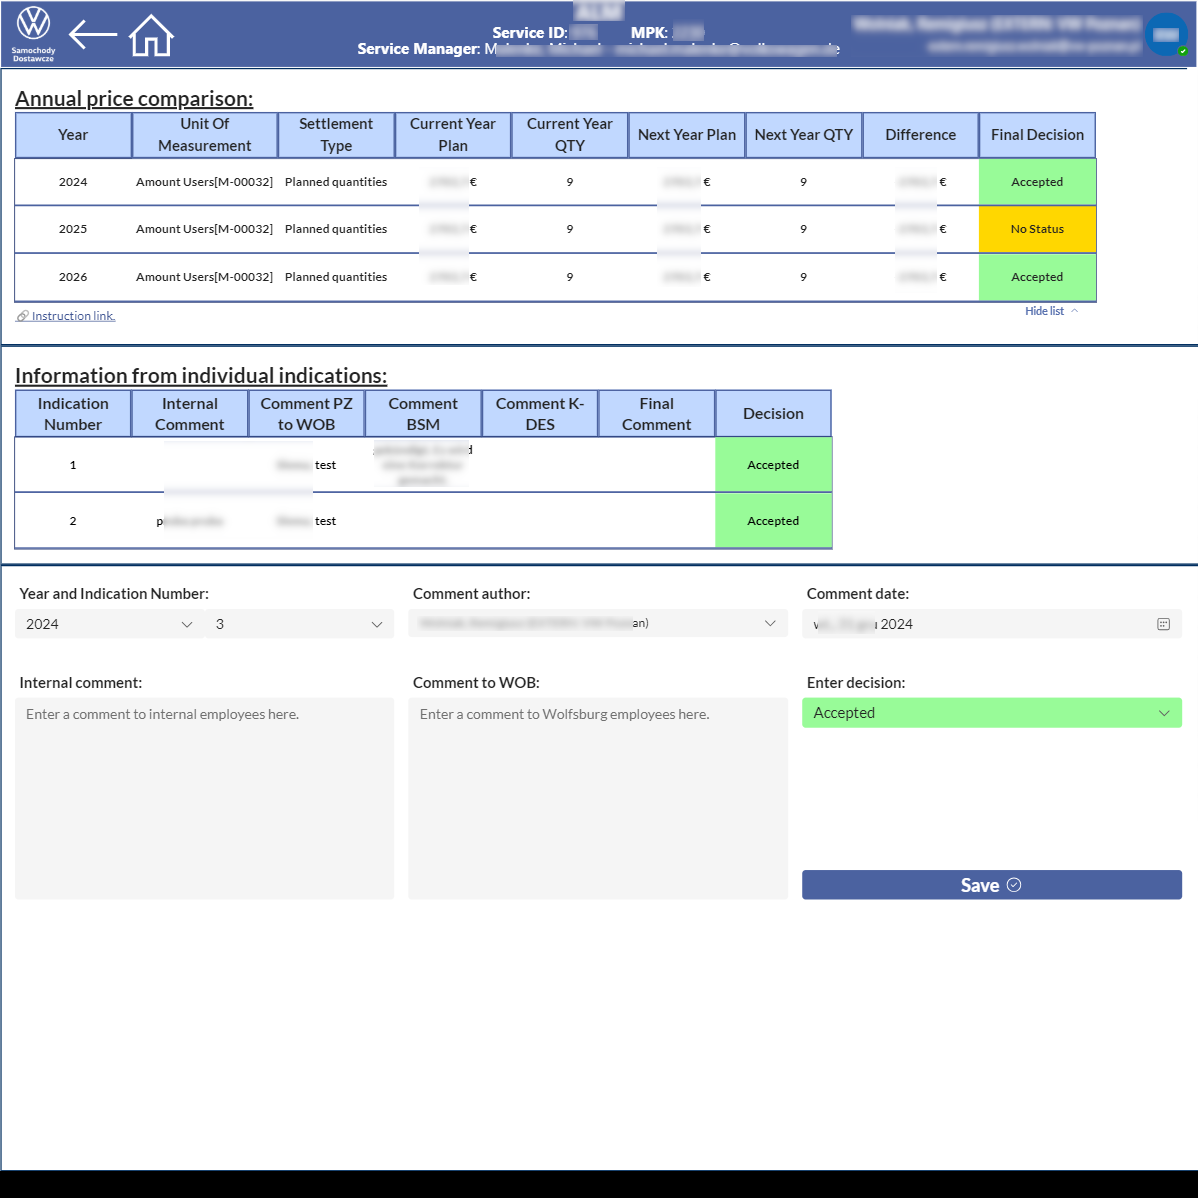
\includegraphics[width=0.9\textwidth]{figures/EditForm.png}
    \caption{Ekran edycji elementu}  
    \label{fig:EditForm}
\end{figure}
\subsubsection{Porównanie finalnych decyzji z poprzednich lat}
W górnej części ekranu znajduje się tabela przedstawiająca porównanie danych finansowych oraz decyzji z trzech ostatnich lat. Dane te są automatycznie pobierane i zawierają:
\begin{itemize}
    \item {Rok (Year)} -- okres, którego dotyczy dana decyzja,
    \item {Jednostka miary (Unit Of Measurement)} -- zazwyczaj ilość licencji. \customnote{w sumie to czasem było niecałkowite to idk}
    \item {Zeszłoroczne i planowane na następny rok wartości finansowe} -- np. \textit{Current Year Plan} oraz \textit{Next Year Plan},
    \item {Różnice w finansach (Difference)} -- różnica między zeszłorocznymi i potencjalnymi przyszłymi kosztami,
    \item {Status końcowej decyzji (Final Decision)} -- decyzje dotyczące planów z danego roku (\textit{Accepted, Not Accepted, No Status}).
\end{itemize}

Sekcja ta pozwala użytkownikowi przeanalizować ostatnie decyzje oraz ocenić trendy finansowe dla danej usługi w kolejnych latach.

\subsubsection{Link do instrukcji obsługi}
Poniżej tabeli z porównaniem decyzji znajduje się link do dedykowanej instrukcji obsługi usługi. Za pomocą linku użytkownik posiada dostęp do szczegółowych informacji na temat zasad korzystania z danej usługi, co może być przydatne podczas edycji danych lub wprowadzania nowych decyzji.

\subsubsection{Porównanie tegorocznych indykacji}
Sekcja ta prezentuje szczegóły kolejnych indykacji w ramach bieżącego roku. Użytkownik może zobaczyć i analizować szczegóły poszczególnych indykacji, takich jak:
\begin{itemize}
    \item {Numer indykacji (Indication Number)} -- \customnote{\textbf{??? wtf ->} numer kolejny przypisany do konkretnej decyzji},
    \item {Komentarze} -- w tym \textit{Internal Comment, Comment PZ to WOB, Comment K-DES}, które umożliwiają przekazanie informacji pomiędzy działami,
    \item {Data i autor komentarza} -- \customnote{\textbf{tutaj umo też zbędne bo chyba nie trzeba tłumaczyć że autor komentarza to autor komentarza a data komentarza to data komentarza nie?} dane dotyczące daty wprowadzenia decyzji oraz osoby odpowiedzialnej},
    \item {Status decyzji (Decision)} -- użytkownik może zobaczyć, czy decyzja została zaakceptowana (\textit{Accepted}), odrzucona (\textit{Not Accepted}) lub jeszcze nie podjęta (\textit{No Status}).
\end{itemize}

\subsubsection{Formularz do uzupełnienia danych}
Na samym dole strony znajduje się formularz umożliwiający wprowadzenie nowych danych lub aktualizację istniejących rekordów. Formularz zawiera pola takie jak:
\begin{itemize}
    \item {Rok (\textit{Year})} -- użytkownik może wybrać rok, którego dotyczy wpis,
    \item {Numer indykacji (\textit{Indication Number})} -- kolejny numer przypisany do decyzji,
    \item {Komentarze} -- pola do wprowadzenia uwag wewnętrznych, komentarzy między działami oraz końcowych komentarzy,
    \item {Status decyzji (\textit{Decision})} -- lista rozwijana, umożliwiająca wybór odpowiedniego statusu (\textit{Accepted, Not Accepted, No Status}),
    \item {Data i autor} -- data oraz osoba odpowiedzialna za wprowadzenie wpisu.
\end{itemize}

Przycisk \textit{Save} umożliwia zapisanie wprowadzonych zmian. Mechanizm ten:
\begin{itemize}
    \item Sprawdza istnienie wcześniejszych indykacji, aby upewnić się, że zachowana jest poprawna kolejność numeracji,
    \item W przypadku istniejącego wpisu -- aktualizuje dane (\textit{Patch}),
    \item W przypadku nowego wpisu -- tworzy nowy rekord (\textit{Defaults}),
    \item Resetuje pola formularza oraz odświeża dane na ekranie, aby uwzględnić ostatnie zmiany,
    \item Informuje użytkownika o powodzeniu lub błędach operacji za pomocą komunikatów (\textit{Notify}).
\end{itemize}

\subsubsection{Podsumowanie}
\customnote{\textbf{To to chyba do rozdziału 'Podsumowanie' bedzie co?}
    Ekran edycji elementu został zaprojektowany tak, aby umożliwić użytkownikom zarówno przeglądanie historycznych danych finansowych, jak i łatwe wprowadzanie nowych decyzji lub modyfikację istniejących. Dzięki logicznemu układowi sekcji oraz dynamicznej aktualizacji danych, interfejs wspiera efektywne zarządzanie informacjami dla każdej usługi.}
\end{comment}
\section{Edycja danych}

Po zapisaniu najnowszych danych, kolejnym krokiem jest wprowadzenie niezbędnych aktualizacji dotyczących usług. W tym celu zaimplementowano dwa ekrany: pierwszy służy do wyboru usługi z listy, a drugi umożliwia przeglądanie i edycję szczegółów związanych z wybraną usługą. Oba ekrany zostały zaprojektowane z myślą o intuicyjnej nawigacji i efektywnym zarządzaniu danymi.

\subsection{Ekran wyboru usługi do edycji}

\begin{figure}[h]
\centering
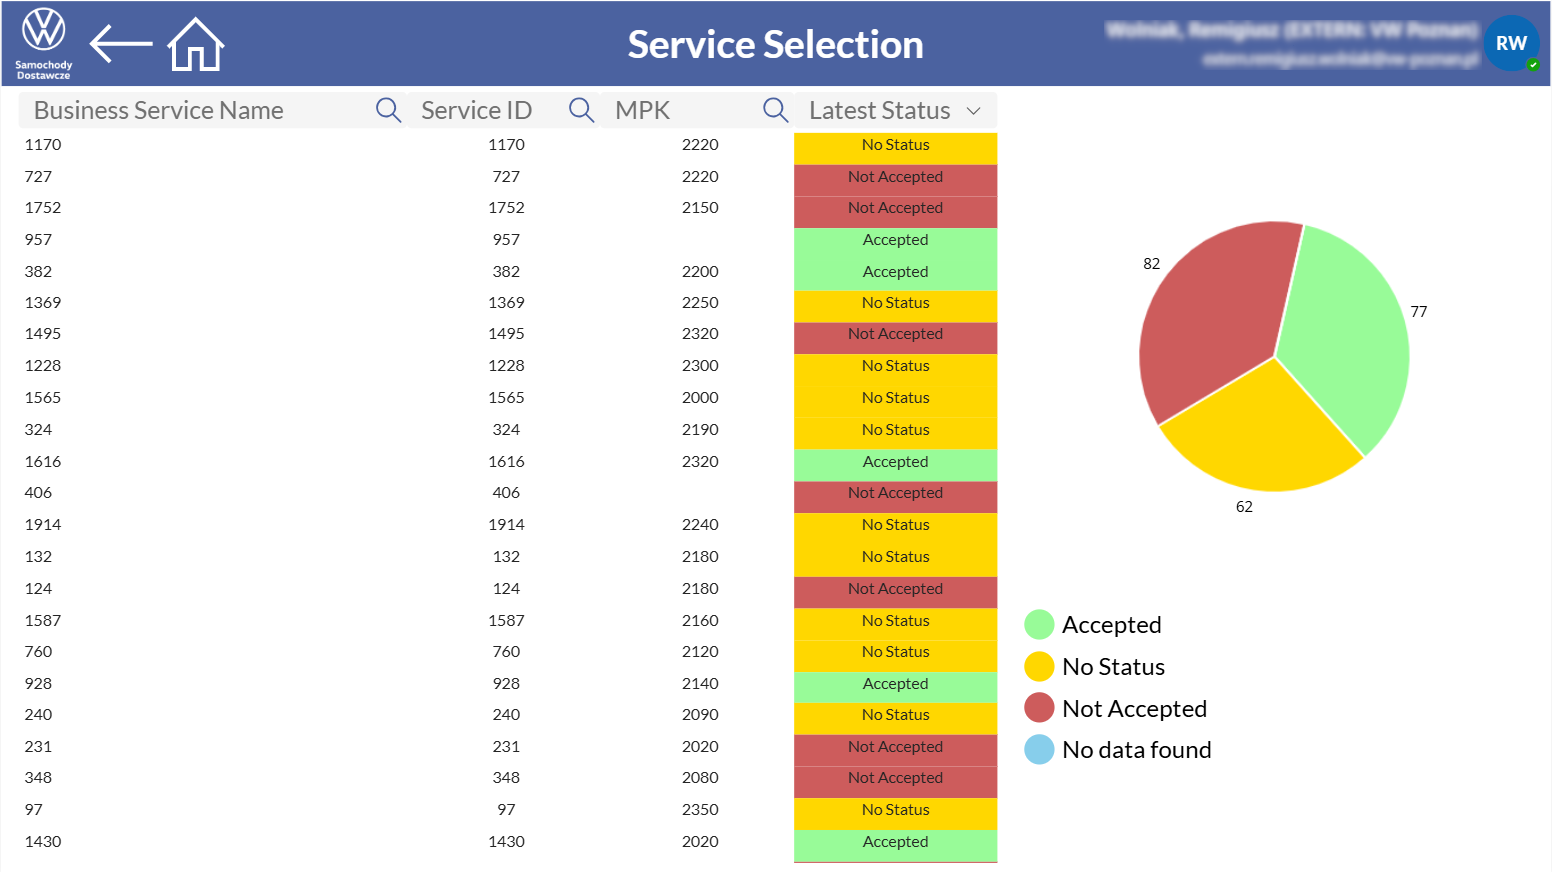
\includegraphics[width=0.9\textwidth]{figures/ServiceSelectionForm.png}
\caption{Ekran wyboru usługi do edycji}
\label{fig:ServiceSelectionForm }
\end{figure}

Ekran wyboru usługi do edycji został zaprojektowany w sposób umożliwiający użytkownikom szybkie i precyzyjne wyszukiwanie oraz filtrowanie danych. Składa się z następujących elementów:

\subsubsection*{Lista wyboru serwisu}

Lista prezentuje dane pochodzące z dynamicznej kolekcji \textit{MergedData}, która została szczegółowo omówiona w poprzednim podrozdziale. Kolekcja ta zawiera zintegrowane informacje z trzech list SharePoint: \textit{Lista\_Uslug}, \textit{Lista\_Kwot} oraz \textit{Lista\_Indykacji}, co umożliwia wyświetlanie najnowszych rekordów, takich jak najświeższe decyzje i kwoty. Dzięki temu użytkownicy mają dostęp do aktualnych informacji bez konieczności ręcznego przeszukiwania źródłowych list.

Każdy element na liście posiada dodatkową funkcję interakcji. Po najechaniu kursorem na wybraną usługę (funkcja \textit{hover}), element wizualnie zmienia swój wygląd — zwęża się, zmienia kolor oraz staje się możliwy do kliknięcia. Kliknięcie przenosi użytkownika do dedykowanego ekranu edycji, który umożliwia szczegółowe zarządzanie wybraną usługą. Ta interaktywność zapewnia intuicyjną nawigację i szybki dostęp do potrzebnych danych.

\subsubsection*{Pola wyszukiwania i filtry}

Użytkownik ma możliwość zawężenia widocznych danych poprzez zastosowanie różnych kryteriów wyszukiwania. Pola obejmują:

\begin{itemize}
\item \textbf{Wyszukiwanie po nazwie usługi (\textit{Service Name})} — Obsługuje częściowe dopasowania dzięki wbudowanej funkcji \textit{StartsWith}, która sprawdza, czy ciąg tekstowy zaczyna się od określonej frazy.
\item \textbf{Filtrowanie po identyfikatorze usługi (\textit{Service ID})} — Umożliwia precyzyjne wyszukiwanie konkretnego elementu.
\item \textbf{Filtrowanie według miejsca powstawania kosztów (\textit{MPK})} — Pozwala na szybkie odnalezienie danych przypisanych do konkretnego obszaru finansowego.
\item \textbf{Filtrowanie według statusu decyzji (\textit{Accepted}, \textit{Not Accepted}, \textit{No Status})} — Dzięki zastosowaniu funkcji \textit{Switch}, wartości statusów są mapowane na odpowiednie kody liczbowe, co ułatwia filtrowanie.
\end{itemize}

Filtry te mogą być stosowane jednocześnie, co umożliwia precyzyjne dopasowanie wyświetlanych danych.

\subsubsection*{Wykres kołowy}

Wykres kołowy ilustruje podział danych według statusów decyzji. Każdy segment odpowiada liczbie elementów z przypisanym statusem, co pozwala użytkownikowi szybko ocenić proporcje między kategoriami (\textit{Accepted}, \textit{Not Accepted}, \textit{No Status}). Wykres jest dynamiczny — aktualizuje się w czasie rzeczywistym w oparciu o zastosowane filtry, co zapewnia aktualność prezentowanych informacji.

\subsection{Ekran edycji elementu}

Ekran edycji elementu, widoczny na rysunku \ref{fig:EditForm }, prezentuje szczegółowe informacje dotyczące wybranej usługi, umożliwiając analizę danych historycznych oraz wprowadzanie nowych decyzji. Ekran składa się z kilku logicznie ułożonych sekcji, które są opisane poniżej.

\begin{figure}[h]
\centering
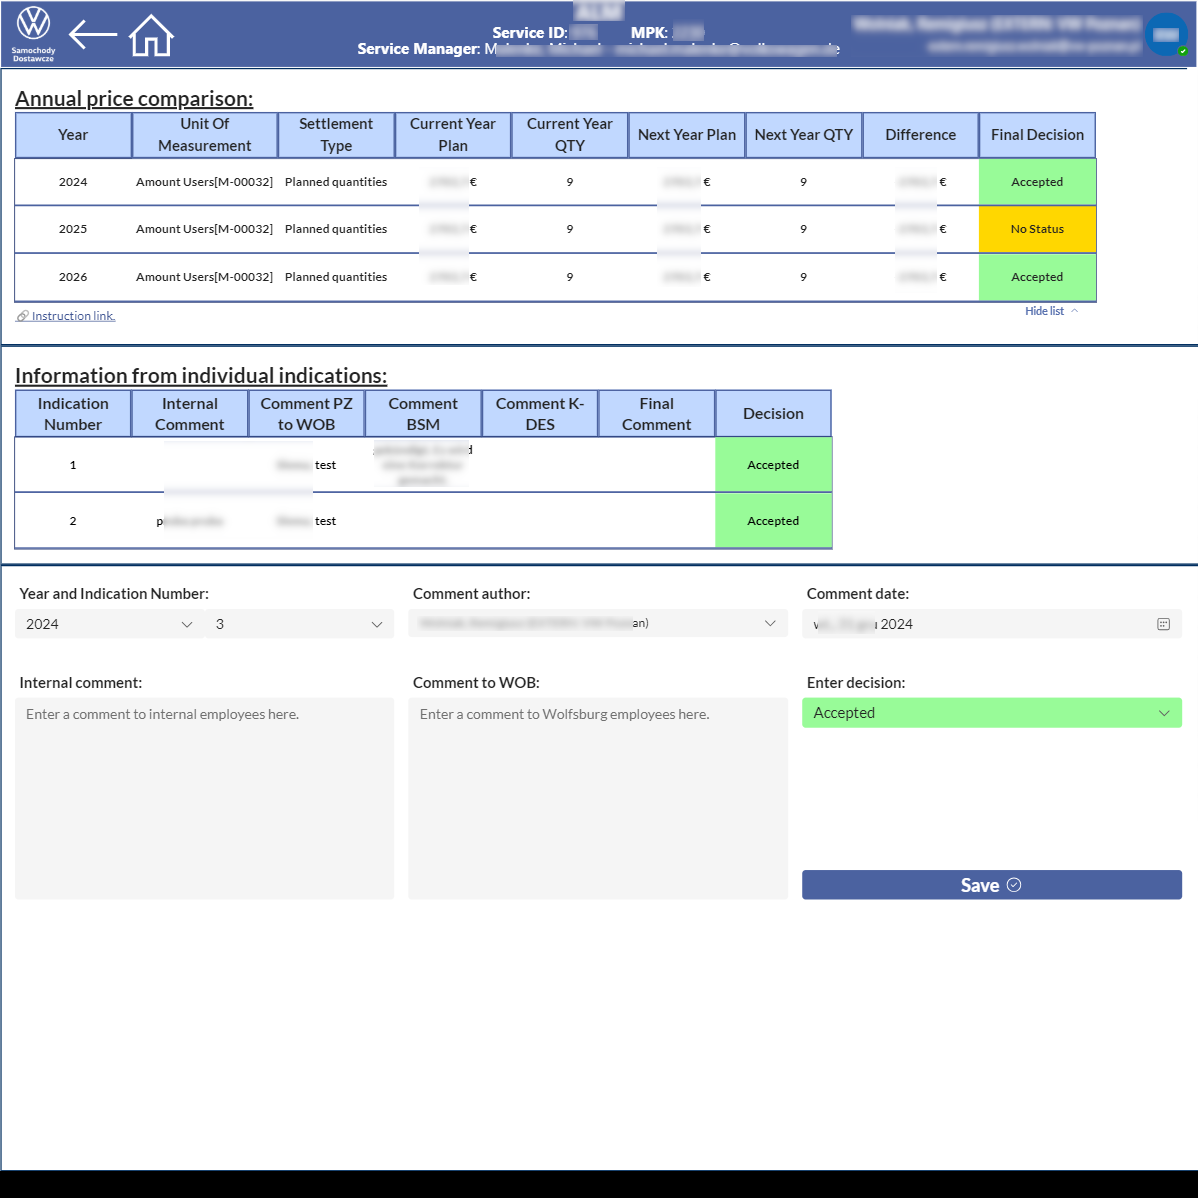
\includegraphics[width=0.9\textwidth]{figures/EditForm.png}
\caption{Ekran edycji elementu}
\label{fig:EditForm }
\end{figure}

\subsubsection{Porównanie finalnych decyzji z poprzednich lat}

W górnej części ekranu znajduje się tabela przedstawiająca porównanie danych finansowych oraz decyzji z trzech ostatnich lat. Dane te są automatycznie pobierane i zawierają:

\begin{itemize}
\item \textbf{Rok (Year)} — okres, którego dotyczy dana decyzja.
\item \textbf{Jednostka miary (Unit Of Measurement)} — zazwyczaj ilość licencji.
\item \textbf{Zeszłoroczne i planowane na następny rok wartości finansowe} — np. \textit{Current Year Plan} oraz \textit{Next Year Plan}.
\item \textbf{Różnice w finansach (Difference)} — różnica między zeszłorocznymi i potencjalnymi przyszłymi kosztami.
\item \textbf{Status końcowej decyzji (Final Decision)} — decyzje dotyczące planów z danego roku (\textit{Accepted, Not Accepted, No Status}).
\end{itemize}

Sekcja ta pozwala użytkownikowi przeanalizować ostatnie decyzje oraz ocenić trendy finansowe dla danej usługi w kolejnych latach.

\subsubsection{Link do instrukcji obsługi}

Poniżej tabeli z porównaniem decyzji znajduje się link do dedykowanej instrukcji obsługi usługi. Za pomocą linku użytkownik posiada dostęp do szczegółowych informacji na temat zasad korzystania z danej usługi, co może być przydatne podczas edycji danych lub wprowadzania nowych decyzji.

\subsubsection{Porównanie tegorocznych indykacji}

Sekcja ta prezentuje szczegóły kolejnych indykacji w ramach bieżącego roku. Użytkownik może zobaczyć i analizować szczegóły poszczególnych indykacji, takie jak:

\begin{itemize}
\item \textbf{Numer indykacji (Indication Number)} — kolejny numer przypisany do konkretnej decyzji.
\item \textbf{Komentarze} — w tym \textit{Internal Comment, Comment PZ to WOB, Comment K-DES}, które umożliwiają przekazanie informacji pomiędzy działami.
\item \textbf{Data i autor komentarza} — informacje dotyczące daty wprowadzenia decyzji oraz osoby odpowiedzialnej.
\item \textbf{Status decyzji (Decision)} — użytkownik może zobaczyć, czy decyzja została zaakceptowana (\textit{Accepted}), odrzucona (\textit{Not Accepted}) lub jeszcze nie podjęta (\textit{No Status}).
\end{itemize}

\subsubsection{Formularz do uzupełnienia danych}

Na samym dole strony znajduje się formularz umożliwiający wprowadzenie nowych danych lub aktualizację istniejących rekordów. Formularz zawiera pola takie jak:

\begin{itemize}
\item \textbf{Rok (\textit{Year})} — użytkownik może wybrać rok, którego dotyczy wpis. Domyślnie pole to jest ustawiane na bieżący rok.
\item \textbf{Numer indykacji (\textit{Indication Number})} — kolejny numer przypisany do decyzji. Numer ten jest automatycznie ustawiany na o jeden większy niż najwyższy numer indykacji dla danego roku w bazie danych.
\item \textbf{Komentarze} — pola do wprowadzenia uwag wewnętrznych, komentarzy między działami oraz końcowych komentarzy.
\item \textbf{Status decyzji (\textit{Decision})} — lista rozwijana, umożliwiająca wybór odpowiedniego statusu (\textit{Accepted, Not Accepted, No Status}). Domyślnie status jest ustawiany na podstawie decyzji z poprzedniego roku.
\item \textbf{Data i autor} — data oraz osoba odpowiedzialna za wprowadzenie wpisu. Pole autora jest automatycznie uzupełniane danymi aktualnie zalogowanego użytkownika.
\end{itemize}

Przycisk \textit{Save} umożliwia zapisanie wprowadzonych zmian. Mechanizm ten:

\begin{itemize}
\item Sprawdza istnienie wcześniejszych indykacji, aby upewnić się, że zachowana jest poprawna kolejność numeracji.
\item W przypadku istniejącego wpisu — aktualizuje dane przy użyciu funkcji \textit{Patch}.
\item W przypadku nowego wpisu — tworzy nowy rekord przy użyciu funkcji \textit{Defaults}.
\item Resetuje pola formularza oraz odświeża dane na ekranie, aby uwzględnić ostatnie zmiany.
\item Informuje użytkownika o powodzeniu lub błędach operacji za pomocą komunikatów (\textit{Notify}).
\end{itemize}

\subsection{Listing kodu}

Listing \ref{lst:SaveFormCode} przedstawia fragment kodu odpowiedzialny za zapisywanie danych w formularzu edycji, który jest wywoływany po kliknięciu przycisku \textit{Save}. Kod ten odpowiedzialny jest za zapisanie informacji z formularza w bazie danych.

\begin{lstlisting}[language=PowerFx, caption={Kod zapisywania danych w formularzu edycji}, label=lst:SaveFormCode ]
    If(
        // Dla indykacji nr 1
        IndicationNo_Dropdown.Selected.Value = 1;
        
        // Sprawdź; czy istnieje już pierwsza indykacja
        If(
            !IsBlank(
                LookUp(
                    Lista_Indykacji;
                    Year = Year_Dropdown.Selected.Value &&
                    IndicationNo = 1 &&
                    Service_ID = ChosenServiceID
                )
            );
            // Aktualizacja istniejącego rekordu
            Set(
                TempOutput;
                Patch(
                    Lista_Indykacji;
                    LookUp(
                        Lista_Indykacji;
                        Year = Year_Dropdown.Selected.Value &&
                        IndicationNo = 1 &&
                        Service_ID = ChosenServiceID
                    );
                    {
                        Comment_date: Text(CommentDateInput.SelectedDate);
                        Comment_author: ComboboxCanvas1.Selected.DisplayName;
                        Comment_PZ_to_WOB: CommentToWOBInput.Value;
                        Comment_Intern: InternalCommentInput.Value;
                        Decision: Switch(
                            DropdownCanvas1.Selected.Value;
                            "Accepted"; 1;
                            "No Status"; 0;
                            "Not Accepted"; -1;
                            0
                        )
                    }
                )
            );;
            Notify("A record has been successfully updated!"; NotificationType.Success);
            
            // Jeśli rekord nie istnieje; utwórz nowy
            Set(
                TempOutput;
                Patch(
                    Lista_Indykacji;
                    Defaults(Lista_Indykacji);
                    {
                        Service_ID: ChosenServiceID;
                        Year: Year_Dropdown.Selected.Value;
                        IndicationNo: 1;
                        Comment_date: Text(CommentDateInput.SelectedDate);
                        Comment_author: ComboboxCanvas1.Selected.DisplayName;
                        Comment_PZ_to_WOB: CommentToWOBInput.Value;
                        Comment_Intern: InternalCommentInput.Value;
                        Decision: Switch(
                            DropdownCanvas1.Selected.Value;
                            "Accepted"; 1;
                            "No Status"; 0;
                            "Not Accepted"; -1;
                            0
                        )
                    }
                )
            );;
            Notify("The record has been successfully created!"; NotificationType.Success)
        )
    );;    
\end{lstlisting}